\documentclass[11pt]{report}

\usepackage{fancyhdr} % Cabeceras de página
\usepackage{lastpage} % Módulo para añadir una referencia a la última página
\usepackage{titling} % No tengo claro para qué es esto
\usepackage[left=3cm,right=2.5cm,top=3cm,bottom=2cm]{geometry} % Márgenes
\usepackage[T1]{fontenc}
\usepackage[utf8x]{inputenc}
\usepackage{xspace}
\usepackage{graphicx}
\usepackage{tikz}
\usepackage{wrapfig}
\usepackage{hyperref}
\usepackage{amssymb}
\usepackage{multirow}
\usepackage[official]{eurosym}

\hypersetup{
  	hyperindex,
    colorlinks,
    allcolors=blue!60!black
}


\setcounter{secnumdepth}{3}
\renewcommand{\baselinestretch}{1.4}

\title{UAM Software Notification and Damage Management System \\ Project Plan}
\date{\today}
\author{{\Large Triforce} \\ \vspace{5pt} \textit{Iván Márquez Pardo, Víctor de Juan Sanz, Guillermo Julián Moreno}}

\fancyhf{}
\fancypagestyle{plain}{%
	\lhead{\raisebox{12pt}{\textsc{Project Plan} - \small Ref. TFC-UAM-01}}
	\chead{\centering \vspace{-15pt} 
\includegraphics[width =40 pt]{../Logo.jpg}}
	\rhead{\raisebox{12pt}{\small Ver. 1.0 - \today \vspace{2pt}}}
	\cfoot{\thepage\ of \pageref{LastPage}}
	\rfoot{}
}

\newcounter{reqs}[chapter]
\newcounter{NFreqs}[chapter]
\newcommand{\header}[1]{\\ \indent \textbf{#1}\hspace{10pt}}

\newcommand{\reqvertsep}{\vspace{-7pt}}

\newcommand{\reqdesc}{\subparagraph{Description}}
\newcommand{\reqin}{\reqvertsep\subparagraph{Input data}}
\newcommand{\reqout}{\reqvertsep\subparagraph{Output data}}
\newcommand{\reqsteps}{\reqvertsep\subparagraph{Steps}}

\newenvironment{requirement}[1]{
	\subsubsection{\textsc{Functional Requirement \arabic{reqs}} - #1}
	\refstepcounter{reqs}
}{\vspace{20pt}}

\newenvironment{NFrequirement}[1]{
	\subsubsection{\textsc{Non-Functional Requirement \arabic{NFreqs}}}
	\refstepcounter{NFreqs}
}{\vspace{20pt}}

\newcommand{\reqref}[1]{Req. \ref{#1}}

\begin{document}
\maketitle

\begin{table}[hbtp]
\centering
\begin{tabular}{|c|c|p{3cm}|p{3.5cm}|}
\hline \multicolumn{4}{|c|}{\textsc{Version table}} \\ \hline \hline
\textbf{Version} & \textbf{Date} & \textbf{Main changes} & \textbf{Purpose} \\ \hline
\end{tabular}
\end{table}

\begin{description}
\item[Written by] Guillermo Julián Moreno, Víctor de Juan Sanz, Iván Márquez Pardo.
\item[Reviewed by] Guillermo Julián Moreno, Víctor de Juan Sanz, Iván Márquez Pardo (\today).
\item[Approved by] Guillermo Julián Moreno, Víctor de Juan Sanz, Iván Márquez Pardo (\today).
\end{description}

\begin{figure}[hbtp]
\centering

\includegraphics[width=0.8\textwidth]{../Yo.jpg}
\caption{Julián approves.}
\end{figure}


\newpage

\begin{abstract}
\end{abstract}

\tableofcontents
\newpage
\pagestyle{plain}

\chapter{Subsystems and Requirements}
% -*- root: ../ProjectPlan.tex -*-
\section{Project Definition}

FML is based on the jolly cooperation between the users of the facilities of the UAM campus and the maintenance staff in charge of them.

As the users will be the ones that will detect the sooner faults on the facilities the campus offers them, they are also the most suitable to report the problems they are having, in order to getting them fixed as soon as possible. With the FML web application, it will only take less than a minute to fill the form and send it to the maintenance staff.

Using the reports of faults detected in the campus, the maintenance personnel will stop losing its precious time revising the installations looking for faults and will be able to focus on the repairs. Apart from this benefit, the maintenance staff will also have a better way to coordinate efforts, as the FML will provide an automatic assignment system to assign repairs to each of the members avoiding overloading any of them and taking into account their distance to the problem, saving time on displacements.

In summary, the users will be able to easily report faults on facilities they are using in order to have them fixed in the less time possible, while the maintenance personnel will multiply its current performance as the majority of their resources will stop being wasted on revisions, but on repairs. 

\section{Breakdown in Subsystems}

\begin{figure}[hbtp]
\centering
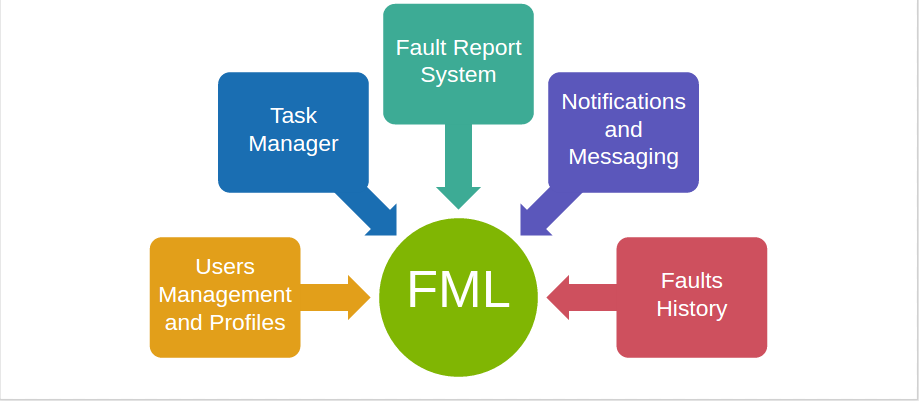
\includegraphics[scale=0.5]{img/subsystems.png}
\caption{Schematic for the subsystems of the project.}
\label{figSubsystems}
\end{figure}

In order to achieve the goals described in chapter \ref{chapIntroduction}, the Fault Manager Lite application is divided into five subsystems: \emph{Task Management}, \emph{Report System}, \emph{Notification and Messaging System}, \emph{User Management} and \emph{Faults History and Statistics}, as seen in figure \ref{figSubsystems}.

A brief description of the functionalities of each mentioned subsystem can be found in the next sections of the document.

\subsection{Task Management}
\label{subsection Task Management}

This subsystem is in charge of the management of repair tasks, which are automatically generated whenever the system receives a new fault report.

Users will use the report system of the application (see \ref{subsection Report System}) to send report faults. These faults will be analyzed by this subsystem and automatically classified depending on their department and priority. Then, their corresponding repair task will be generated based on the form filled by the user and assigned to the closest technician depending on the location of the fault.

Managers will be able to change manually the priority and the person in charge of repairing that fault, which are automatically assigned by the subsystem. The category of the fault can also be modified in case it is not correct; in that case, the fault will then be sent to the manager of the new department. Cleaning department will be treated differently as there is a manager for each building of the UAM campus, so cleaning tasks will be assigned to those managers taking into account this characteristic.

Technicians who have been assigned a repair task will be notified (see \ref{subsection Notification and Messaging System}) and be able to consult the information related to that task. This task information includes: ID of the reporter, location of the fault, timestamp of the report, brief description (subject), detailed description, category, status, priority and occasionally a photography (if any was given by the reporter).

The status of a fault can be: \emph{Pending} (just received by the system, before having been automatically assigned by the system or manually assigned by a manager), \emph{Assigned} (already assigned to a technician, who is or will be eventually solving it) or \emph{Solved} (the task has been successfully completed as the fault has been repaired). Technicians will be able to change the current status of a task assigned to them in order to give managers real-time information about the status of faults' troubleshooting.

Managers will also be able to consult real-time information about repair tasks assigned to members of their departments and make reassignments of tasks in case, for example, of overloading a certain technician or in order to accelerate an specific repair.

\subsection{Report System}
\label{subsection Report System}

This subsystem is in charge of the fault report system, which is the main and most important activity of the whole software system.

Whenever users and/or technicians encounter a fault on the facilities of the campus, they will be able to fill a form in order to report that fault and accelerate its troubleshooting. This fault will then be sent to the FML server, which will assign its repair task to the corresponding technician (see \ref{subsection Task Management}).

The mandatory fields of the form include: a brief description of the problem (subject), a more detailed description (1000 characters maximum length), category (department of the maintenance service) and location (which can be automatically set using GPS technology or manually set by the user in case the GPS function doesn't work properly). The ID of the reporter and the timestamp of the report will be automatically added before sending it.

As an optional field, users can add a photography to their report in case they want to be more specific. The photo will be taken on the fly or added from the user's gallery.

After sending a fault report, the reporter will be able to consult the real-time status of its repair task by selecting that task from his/her fault history (see \ref{subsection Fault History and Statistics}). Reporting a fault enables the opening of a chat conversation with the technician assigned to the repair (see \ref{subsection Notification and Messaging System}).

The report system is also in charge of analyzing newly received fault reports and determine if they can be duplicates of existing reports, by comparing their characteristics: location, similar timestamps and same keywords in the descriptions. Potential duplicates will be sent to the manager, who will decide if they really are the same issue or not.

\subsection{Notification and Messaging System}
\label{subsection Notification and Messaging System}
This subsystem is the one in charge of sending and receiving notifications and messages from the application.

There will exist general and emergency notifications (such as special events in the campus and a fire or blackout in a building, respectively). This notifications will only be sent by managers and all the users will receive that alerts.

Technicians will receive a notification informing them of their assignment of a new task. They will also be able to establish a communication channel (private chat) with the reporter of a fault, in order to ask for more information about that fault. Users will not be able to open this communication channel with the technician in charge of their reported fault, while managers will be able to open a private chat with any member of their departments for a better management and organization of them.

When a fault is repaired and the technician changes its status to solved (see \ref{subsection Task Management}), its reporter will receive a notification about the finish of the repair.

Users and technicians will be able to delete messages or notifications they have received.

\subsection{User Management}
\label{subsection User Management}

This subsystem is in charge of several issues related to the application users, including login, user profile and user's fault history.

In this section, the term `user' will make reference to every member of the UAM that uses the FML application as a reporter or as a member of the maintenance service.

When entering the application, users must introduce their credentials for accessing the UAM's web services. Those credentials will be sent to the UAM members server, which will inform the FML server about the correctness (or not) of them. Login credentials will only be needed once (the first time you access to the application).

Every user will have a profile, including some (optionally filled) information about them. From this profile, every user will have access to their fault report history; every report can be selected in order to see its current status (see \ref{subsection Fault History and Statistics}).

In case of students, this profile will also show them information about their current progress in the achievement of optional credits as a reward for their report history.

This system is also in charge of filtering and/or searching for users in the database. This ability to look for users in the database is only accessible to managers.

\subsection{Fault History and Statistics}
\label{subsection Fault History and Statistics}

This subsystem is in charge of several activities related to fault reports, including their search and the generation of statistics related to them.

When a fault is reported (see \ref{subsection Report System}), that report is saved in the database and its entry can be eventually change. For example, its status will be eventually changed when it gets repaired by a technician, it can be assigned to another technician or its priority can be modified by a manager (see \ref{subsection Task Management}).

Managers will be able to consult the fault database to look for all its entries or apply some filters to look for specific faults. Among the filters that can be applied in the search, there are: category/department, date range, reporter, technician or keyword in the description.

User profiles will make accessible information about fault reports related to those users: reporters will see the faults they have reported and their real-time status, while technicians will see the faults they have repaired or have been assigned to do so. Managers will have all this information available by applying the corresponding filter.

Managers will also be able to generate statistics based on the fault history contained in the database. This statistics can be general, related to their departments or related to a member of their technical staff. The generated statistics can be used to analyze the troubleshooting efficiency of the maintenance service or detect problematic areas.

Users will be able to see a simplified map of the campus with colored signs on it. Each dot represents a reported fault and the color will follow a color code, making its status easily distinguishable depending on it: Pending to assign (red), Assigned (yellow) and Solved (Solved). Only the last 30 reports will be shown in this map at the same time to ensure their visibility.


% -*- root: ../ProjectPlan.tex -*-

\chapter{Requirements}
\label{chapRequirements}

The functional and non-functional requirements of the Fault Manager Lite application are gathered in the next sections of the document.

Functional requirements are organized into their corresponding subsystems. If any requirement could depend on two or more subsystems due to the function it performs, then one of those subsystems (usually the most relevant) will be chosen.

In a similar way, non-functional requirements are organized into categories attending to their scope.

\section{Functional Requirements}

\subsection{Task Management}

\begin{requirement}{Generate repair task}
\reqdesc When the report system receives a new fault report, it will analyze the information it contains in order to generate its corresponding repair task. This task will later be automatically assigned to a technician.
\reqin The fault report sent by an user of the application.
\reqsteps The system will analyze the information of this fault report and generate its corresponding repair task. That task will be classified depending on its category and priority, and saved in the fault database.
\reqout The generated repair task, whose status will be 'Pending'.
\end{requirement}

\begin{requirement}{Visualize new notices of incidences}
\reqdesc Managers will be able to see new notices of incidences that have not been assigned yet, in order to revise their correctness.
\reqin Function triggered manually by the manager by selecting its corresponding option.
\reqsteps Depending on the department the manager is in charge of, the system will look in the fault database for new notices of incidences of that department that are still not solved nor assigned to any technician.
\reqout The system will display a list of incidence reports. Information about each report will also be shown to see their correctness.
\end{requirement}

\begin{requirement}{Definition of priority criteria}
\reqdesc The system must allow to specify different criteria to assign automatically a priority to each incidence.
\reqin The user selects parameters of the incidence object and corresponding keywords that will conform the selection criteria, and the desired priority that will be set on match.
\reqsteps The system stores the criteria and applies it automatically on incidence creation in order to establish a priority.
\reqout The system automatically classifies each incidence based on user-defined criteria: if a certain parameter (e.g., location or description) contains the keywords specified, the priority will be set to whatever the user specified in the criteria.
\end{requirement}

\begin{requirement}{Management of priorities by managers}
\reqdesc Managers must be able to receive reports and manage the incidences based on the departments they are in charge of.
\reqin The maintenance personnel sends messages and incidences to the system.
\reqsteps The system saves all the information and shows them to the personnel in charge.
\reqout Managers sees all related messages and reports.
\end{requirement}

\begin{requirement}{Changes of incidence state}
\reqdesc Managers must be able to change the state (Pending, Assigned or Solved) of each incidence of their departments.
\reqin The manager introduces the new state of the incidence.
\reqsteps The system saves the new state in the database.
\reqout The incidence has the new state registered.
\end{requirement}

\begin{requirement}{Changes of incidence category}
\reqdesc Managers must be able to change the category of each incidence.
\reqin The personnel in charge inputs the new category of the incidence.
\reqsteps The system saves the new category.
\reqout The incidence has the new category registered.
\end{requirement}

\begin{requirement}{Reassignment of tasks}
\reqdesc Managers must be able to change the technician assigned to a repair task.
\reqin The manager has to select a repair task from his/her department and introduce the identifier of other member of his/her department
\reqsteps The system will look into the staff database for the identifier of the new technician and update the corresponding field in the selected repair task.
\reqout Changes in the database entry of the repair task will be saved. The new technician will receive a notification of the new task he/she is in charge of; the previous technician will also receive a task canceling notification.
\end{requirement}

\begin{requirement}{Modify notices of incidences}
\reqdesc Managers will be able to modify reports of incidences for their departments in order to correct any mistake or complete gaps in the forms.
\reqin The manager will be able to change any of the fields (except for the identifier) of a fault report by introducing new information or modifying the existing one. Among the modifiable fields of the report, there will be: title, description, location (in case automatic allocation has failed), category and priority. Confirmation will be needed to save changes.
\reqsteps The system will update in the faults database the data given/modified by the manager. All the modifications of the report will be done within a transaction, and only be applied if the manager confirms so when he/she finishes the process.
\reqout Changes on the fault database will be committed becoming permanent (successful transaction) and the manager will be notified with a confirmation message on the screen.
\end{requirement}

\begin{requirement}{Manual assignment of incidences}
\reqdesc Managers of each department will be able to assign the reparation of incidences to technical members of their department.
\reqin The manager will have to introduce the identifier of the fault report and the name/identifier of the technician that will fix that fault.
\reqsteps The system will look for the technician in the staff database and for the fault report in the faults database. The status of the fault will be changed from 'Pending' to 'Assigned' and the fault will now be related to its technician.
\reqout A confirmation message will be shown to the manager and the technician will receive a notification of the new task he/she has been assigned to repair.
\end{requirement}

\begin{requirement}{Automatic assignment of incidences}
\reqdesc The system will automatically assign repair tasks whose status is 'Pending' to the closest technician from the department of the fault (category).
\reqin A repair task with 'Pending' status.
\reqsteps The system will take the category and location of the reported fault and look for the closest technician that belongs to that department and assign him/her that repair task. The status of the fault will be changed from 'Pending' to 'Assigned' and the fault will now be related to its technician.
\reqout The status of the fault in the database will be changed and the technician will receive a notification of the new task he/she has been assigned to repair.
\end{requirement}

\begin{requirement}{Filtering list of categories}
\reqdesc The system must allow users to search and filter from the category list.
\reqin Logical combination (\textit{and, or, not}) of attribute and value pairs that constitute the filter.
\reqsteps The system validates the filter query, then filters the list of categories according to that filter.
\reqout List of filtered categories.
\end{requirement}

\begin{requirement}{Add new categories}
\reqdesc The system must allow administrators to add new categories.
\reqin Information needed to create category. This information is given by external inputs: title and information of department's chief.
\reqsteps The system ensures that the category does not exist previously before creating it, and then saves the category in the database.
\reqout The department chief object is stored into database and the list of categories is updated.
\end{requirement}

\begin{requirement}{Delete categories}
\reqdesc The system must allow administrators to delete categories.
\reqin The category object to delete.
\reqsteps The system finds the category and every task with the category being deleted. Those tasks are changed removing this category to maintain coherence of the inner system database. Finally, the category is removed from the system.
\reqout The category disappears from the database and from every task categorized with it.
\end{requirement}

\begin{requirement}{Modifying category stored values and its priority}
\reqdesc The system must allow administrators to modify categories attributes and its priority stored.
\reqin The category to be modified and the attributes that are going to be changed.
\reqsteps The system finds the category and changes the corresponding attributes. There's no need to update related objects as the category identification number is not modifiable, except if the priority is modified.

If the priority is modified, the system will update the priority of every task that hasn't been set manually by the users.
\reqout The database is updated with the new information for the category. If the priority for the category is modified, tasks in the system are updated accordingly and the system will notify the users related with those updated tasks.
\end{requirement}


\subsection{Report System}

\begin{requirement}{Fault location}
\label{reqFaultLocation}
\reqdesc Get the location of the fault, based on the location of the reporter.
\reqin Two kind of external inputs are necessary for determine location:
\begin{itemize}
\item Facility where the fault is located, given by.
\subitem GPS coordinates (if possible).
\subitem Manually chose location.
\item Manually chose floor and room inside the building where the fault is located.
\end{itemize}
\reqsteps Transform input information into Location object.
\reqout Location object.
\end{requirement}

\begin{requirement}{Incidences report}\label{ReportSystem_IncidencesReport}
\reqdesc The system must allow users to report incidences.
\reqin The user must input a title and a category for the report. The system will automatically set a location for the report (\reqref{reqFaultLocation}). Optionally, the user can add a description of the problem and a picture. The system will send also the identification of the user who's reporting the task.
\reqsteps The system generates an object with all the information given by the reporter. The system adds additional calculated information such as priority (decided automatically based on category).
\reqout The fault reported object.
\end{requirement}

\begin{requirement}{Store incidences report}
\reqdesc Store into database the report object given by \ref{ReportSystem_IncidencesReport}
\reqin Report object.
\reqdesc The system saves in the database a new record with the input data and the user who reported it.
\reqout The reported fault object is stored into the database, and the maintenance personnel is notified of the new fault. The user receives an acknowledgment of the received report.
\end{requirement}

\subsection{Notification and Messaging System}

\begin{requirement}{Notification when the fault has been solved}
\reqdesc The user will receive a notification when a fault he has reported has been solved.
\reqin Reported fault object and the user who will receive the notification.
\reqsteps The system retrieves the notification preferences for the user (e.g., mail, push mobile notification), builds the notification and sends it through the corresponding external channel.
\reqout A message saying the fault has been solved successfully with a brief summary of it is sent to the user.
\end{requirement}

\begin{requirement}{Receive general notifications}\label{ReqRcvNotif}
\reqdesc Users of the application will receive notifications of general purpose that have been sent by administrators. Among these notifications we can find for example: new version of the app, fire or blackout in a building, special events in the campus, etc.
\reqin A new notification has been send by a manager.
\reqsteps The system will look for the new notification in the database and show it to the user.
\reqout The notification will be displayed to the user.
\end{requirement}

\begin{requirement}{Send general notifications}
\reqdesc Manager will be able to write notifications of general purpose and send them to the users of the application. Among these notifications we can find for example: new version of the app, fire or blackout in a building, special events in the campus, etc.
\reqin The manager has to write a notification message.
\reqsteps The system will get that message and store it in the database. Then, it will alert the client applications of the existence of a new notification.
\reqout The message has been stored in the database so all the users will be able to receive it later (see \ref{ReqRcvNotif}).
\end{requirement}

\begin{requirement}{Send messages to users}
\reqdesc Users will be able to send messages to other users following the some limitations: managers and technicians can send messages to each other and/or to the reporter of an incidence; the reporter of an incidence can only send messages to the technician assigned to that fault, only if the technician has contacted him/her before (the technician has started the conversation with the reporter).
\reqin The fault report to talk about and the message to send.
\reqsteps The system retrieves the users that should receive the message. Those are the users related to that task (reporters and maintenance personnel) apart from the one who is going to send the message. The message is stored in the system and every user related to that fault report will be able to see it in the chat section of the selected report.
\reqout The message is stored in the system so that all users related to the task can see the new message sent regarding the corresponding report.
\end{requirement}

\begin{requirement}{Read messages of a selected report}
\reqdesc Users will be able to read messages of fault reports they are related to (they are the reporters, assigned technicians or managers of the department the report belongs to).
\reqin The fault report that may contain some messages.
\reqsteps The system will retrieve the messages related to that fault report and show them to the interested user in the chat section of the selected report.
\reqout The messages found in the system (if any) that are related to that fault report.
\end{requirement}

\subsection{User Management}

\begin{requirement}{Login into the system}
\reqdesc Every user can login in the application introducing their credentials for the UAM's identification server, confirming they are recognised members of the university.
\reqin The user's credential for the UAM identification server.
\reqsteps The system will take the credentials given by the user and resend them to the UAM identification server, which will validate or not that credentials. 
\reqout Depending on the answer of that server, the user will access or not into his account in the application.
\end{requirement}

\begin{requirement}{Report a misbehaving user}
\reqdesc When technicians encounter a fake fault report, they can report the user who sent that report as an alert of misbehaviour.
\reqin The identifier of the user to report, that is present in the repair task given to the technician.
\reqsteps The system will look for the user's identifier in the database and send a notification containing that identifier and the fake fault report to the administrator, who will decide if the user must be baned or not. 
\reqout Report notification sent to the administrator.
\end{requirement}

\begin{requirement}{Ban an user from the system}
\reqdesc Administrator are able to ban any user from the application in order to prevent more misbehaving from those users.
\reqin The report notification, sent by a technician. The administrator will decide to ban that user or not for an specific period of time: no ban, one week ban, one month ban, indefinitely ban.
\reqsteps The system will show the report notification sent by a technician and wait for the selection of a ban period of time. 
\reqout The user might be unable to login into the system during the period of time specified by the administrator.
\end{requirement}

\begin{requirement}{See fault history}
\reqdesc Registered users will be able to list the faults they have reported and select one of them.
\reqin The user that wants to see his/her tasks.
\reqsteps The system retrieves the list of faults reported by the given user.
\reqout A list of the reports sent by the given user and ordered by date.
\end{requirement}

\begin{requirement}{Show to a manager the list of members of his/her technical staff}\label{ReqShowTechnicians}
\reqdesc Managers will be able to visualize an interactive list of members of the technical staff they are in charge of. The list will be interactive in the sense that the manager would be able to see more information about an specific technician (see next requirement).
\reqin The manager has to introduce the name and/or the numeric identifier of the technician whose statistics and profile wants to see. Then, the manager will have to select one from the results of the search done.
\reqsteps The system will use the criteria introduced by the manager to look for employees that match them. Then, it will show a list of the matchings and once the manager has chosen one of the list, the system will gather the corresponding information from the staff database (profile info) and the fault database (in order to generate statistics about the chosen technician).
\reqout The system will show the manager the profile of the selected technician. In addition, it will also generate some statistics related to the work performed by that technician.
\end{requirement}

\begin{requirement}{Show detailed information about a technician}
\reqdesc Managers will have available to get more information about any of the technicians that are members of their departments.This information will be in the form of statistics and profiles of the corresponding technicians.
\reqin The manager has to choose one of the technicians from the complete list of members of his/her technical staff (see \ref{ReqShowTechnicians}) whose statistics and profile wants to see.
\reqsteps The system will retrieve the corresponding information about this technician from the staff database (personal and contact information) and the fault database (tasks assigned and solved tasks in order to generate statistics about his/her performance). The statistics generated will include information about (at least) his/her average working time, effectiveness and most common tasks solved.
\reqout The system will show the manager the profile of the selected technician. In addition, it will also generate some statistics related to the work performed by that technician. This information will be given to the manager in the form of a report.
\end{requirement}


\subsection{Fault History and Statistics}

\begin{requirement}{Check history of reported fault}
\reqdesc Registered users will be able to check details of a reported fault.
\reqin Fault reported object with all information attached.
\reqout Report showing all the information attached to the object.
\end{requirement}

\begin{requirement}{Tracking incidence impact}
\reqdesc The system must allow internal users with a maintenance personnel profile to check the impact of the incidences.
\reqin Incidence object associated to the user logged in.
\reqsteps The system retrieves the incidence from the database, specifically the impact saved.
\reqout Numeric value showing the impact of the incidence.
\end{requirement}

\begin{requirement}{Get report of incidences}
\reqdesc Managers will have access to a report on incidences. On one hand this report will show the incidences that are not solved or those that are being solved in order of priority. On the other hand, the incidences report will show in a similar way the last incidences that have been solved, sorted by
their resolution date.
\reqin The manager will trigger this action by selecting its corresponding option.
\reqsteps The system will look into the faults database for fault reports that are not solved or they are being solved at the moment, and will order the results by priority. Then, in the same database, the system will filter by reports already solved and order them by resolution date. With these two sets of results, an interactive report will be produced.
\reqout The system will show the manager the report produced by his/her request. This report is interactive in the sense that the manager can select one of the faults to see its characteristics.
\end{requirement}

\begin{requirement}{List all reports}\label{A4-ListAllReports}
\reqdesc The system must allow listing all reported faults.
\reqin An optional filter that will be applied to the shown faults. The list can be filtered by category, priority or location.
\reqsteps The system will search into the database all reports matching the given values. Those reports will be shown to the user.
\reqout List of the reports matching with given values, ordered first by category and then by date.
\end{requirement}

\begin{requirement}{Review single report}
\reqdesc Users will be able to check details of a reported fault from the full list of reports (given by \ref{A4-ListAllReports}).
\reqin Fault reported object with all information attached.
\reqsteps The system retrieves all the information present in the database related to the selected report.

\reqout Report showing all the information attached to the object.
\end{requirement}


\begin{requirement}{Visualize history of tasks}
\reqdesc Managers will be able to visualize the complete
history of tasks in a table where each row represents an incidence.
\reqin The manager will trigger this function by selecting its corresponding option.
\reqsteps The system will access the incidences database in order to retrieve information about all the faults reported and show it to the manager. By default, the tasks will be ordered by date.
\reqout The system will display in the screen a table containing all the incidences reported until that moment.
\end{requirement}

\begin{requirement}{Sort history of tasks}
\reqdesc Managers will be able to sort the history of tasks depending of different criteria chosen by the manager. This sorting criteria includes at least: priority, category, date, state.
\reqin The complete history of tasks has been previously retrieved. The manager will have to choose a criteria among the list given above.
\reqsteps The system will take the results of the history of tasks it has previously retrieved and order them by the chosen criteria.
\reqout The system will display in the screen a table containing all the incidences sorted in the requested order.
\end{requirement}

\begin{requirement}{Consult extended information about an incidence on the report}
\reqdesc Managers will be able to consult extended information on each of the incidences that appear in the report of incidences.
\reqin Report of incidences produced by the system. The manager will have to select one of the incidences of the report to see detailed information about it.
\reqsteps The system will look into the faults database for the selected fault, gather all the information related to it and show it to the manager.
\reqout The system will show the manager a new screen with detailed information about the incidence he/she has selected in the report.
\end{requirement}

\begin{requirement}{Generate statistics about incidences}
\reqdesc Managers will be able to get statistics related to the tasks and to their related areas will be available in order to
detect problematic areas or departments.
\reqin The manager will trigger this function by selecting its corresponding option.
\reqsteps The system will take all the information about incidences stored in the incidences database in order to analyze it and generate some statistics about them. Relevant information for the statistics will be the category, priority and location of tasks. Statistics will also take into account the costs of the repairs and the time elapsed from the detection of a fault until it has been solved (statistics about effectiveness and efficiency of fault troubleshooting).
\reqout A report containing the statistics generated will be shown to the manager.
\end{requirement}

\begin{requirement}{Print reports/screens}
\reqdesc All the reports generated by the application will be printable. This also applies to new screens that the application opens in order to show any requested information.
\reqin Report or screen that the system has generated or opened by the request of an user.
\reqsteps The system will convert the report or the screen to a PDF document and send it to the printer.
\reqout The printed document.
\end{requirement}


\section{Non-Functional Requirements}



\chapter{System size estimation}
% -*- root: ../ProjectPlan.tex -*-
Estimations of time and complexity of the system are basic in order to make a project plan adjusted to the real development time. On the contrary, we won't have any basis to aproximate that time, depending just on a correct planification guided by previous experiences.

With this aim, the size of the Fault Manager Lite project has been estimated using the Function Points estimation technique. Moreover, we have also estimated the Report System (subsystem of FML) with the COCOMO II tool.

\section{Estimation using function points}
\subsection{Unadjusted Function Points}
After the evaluation of the requirements of the proposed system using the Function Points analysis, we have obtained the data of its estimated complexity. We attach tables with the size of the different subsystems in which the application is divided into, with their corresponding estimations in terms of Function Points. For a more detailed analysis of each of the exposed requirements, see \ref{chapFunctionPoints}.


\subsubsection{Task Management Subsystem}
Table \ref{tbl_TMS_UFP} shows the summary of the unadjusted Function Points calculated for the Task Management Subsystem.
\begin{table}[hbtp]
\centering

\begin{tabular}{|l|c|c|c|c|c|c|c|}
\cline{2-7}
\multicolumn{1}{c}{} & \multicolumn{6}{|c|}{\textsc{Complexity}} & \multicolumn{1}{c}{}  \\ \cline{2-8}
\multicolumn{1}{c|}{} & \textbf{Low} & \textbf{Medium} & \textbf{High} & \textbf{Low} & \textbf{Medium} & \textbf{High} & \multirow{2}{*}{\textit{Unadjusted FP}} \\ \cline{1-7}
\textbf{Data fns.} & \multicolumn{3}{|c|}{\textit{Frequency}} &  \multicolumn{3}{|c|}{\textit{Weight}} & \\ \hline
ILF 	& 11 & 0 & 0 & 7 & 10 & 15 & 77 	\\ \hline
EIF 	& 0 & 0 & 0 & 5 & 7 & 10 & 0		\\ \hline
\textbf{Transactional fns.} & \multicolumn{7}{|c|}{} \\ \hline
EI 		& 0 & 0 & 0 & 3 & 4 & 6 & 0 		\\ \hline
EO 		& 0 & 0 & 0 & 4 & 5 & 7 & 0		\\ \hline
EQ		& 3 & 0 & 0 & 3 & 4 & 6 & 9		\\ \hline
\multicolumn{6}{c|}{} & \textbf{Total} & 86.0 \\ \cline{7-8}
\end{tabular}

\caption{Overview of the calculation of the Unadjusted Function Points for the Task Management Subsystem.}
\label{tbl_TMS_UFP}
\end{table}

\subsubsection{Report System Subsystem}
Table \ref{tbl_RSS_UFP} shows the summary of the unadjusted Function Points calculated for the Report System Subsystem.
\begin{table}[hbtp]
\centering

\begin{tabular}{|l|c|c|c|c|c|c|c|}
\cline{2-7}
\multicolumn{1}{c}{} & \multicolumn{6}{|c|}{\textsc{Complexity}} & \multicolumn{1}{c}{}  \\ \cline{2-8}
\multicolumn{1}{c|}{} & \textbf{Low} & \textbf{Medium} & \textbf{High} & \textbf{Low} & \textbf{Medium} & \textbf{High} & \multirow{2}{*}{\textit{Unadjusted FP}} \\ \cline{1-7}
\textbf{Data fns.} & \multicolumn{3}{|c|}{\textit{Frequency}} &  \multicolumn{3}{|c|}{\textit{Weight}} & \\ \hline
ILF 	& 1 & 0 & 0 & 7 & 10 & 15 & 7 	\\ \hline
EIF 	& 0 & 0 & 0 & 5 & 7 & 10 & 0		\\ \hline
\textbf{Transactional fns.} & \multicolumn{7}{|c|}{} \\ \hline
EI 		& 2 & 0 & 0 & 3 & 4 & 6 & 6		\\ \hline
EO 		& 0 & 0 & 0 & 4 & 5 & 7 & 0		\\ \hline
EQ		& 0 & 0 & 0 & 3 & 4 & 6 & 0		\\ \hline
\multicolumn{6}{c|}{} & \textbf{Total} & 13.0 \\ \cline{7-8}
\end{tabular}

\caption{Overview of the calculation of the Unadjusted Function Points for the Report System Subsystem.}
\label{tbl_RSS_UFP}
\end{table}

\subsubsection{Notification and Messaging System Subsystem}
Table \ref{tbl_NMSS_UFP} shows the summary of the unadjusted Function Points calculated for the Notification and Messaging System Subsystem.
\begin{table}[hbtp]
\centering

\begin{tabular}{|l|c|c|c|c|c|c|c|}
\cline{2-7}
\multicolumn{1}{c}{} & \multicolumn{6}{|c|}{\textsc{Complexity}} & \multicolumn{1}{c}{}  \\ \cline{2-8}
\multicolumn{1}{c|}{} & \textbf{Low} & \textbf{Medium} & \textbf{High} & \textbf{Low} & \textbf{Medium} & \textbf{High} & \multirow{2}{*}{\textit{Unadjusted FP}} \\ \cline{1-7}
\textbf{Data fns.} & \multicolumn{3}{|c|}{\textit{Frequency}} &  \multicolumn{3}{|c|}{\textit{Weight}} & \\ \hline
ILF 	& 1 & 0 & 0 & 7 & 10 & 15 & 7 	\\ \hline
EIF 	& 0 & 0 & 0 & 5 & 7 & 10 & 0		\\ \hline
\textbf{Transactional fns.} & \multicolumn{7}{|c|}{} \\ \hline
EI 		& 0 & 0 & 0 & 3 & 4 & 6 & 0 		\\ \hline
EO 		& 0 & 0 & 0 & 4 & 5 & 7 & 0		\\ \hline
EQ		& 3 & 0 & 0 & 3 & 4 & 6 & 9		\\ \hline
\multicolumn{6}{c|}{} & \textbf{Total} & 16.0 \\ \cline{7-8}
\end{tabular}

\caption{Overview of the calculation of the Unadjusted Function Points for the Notification and Messaging System Subsystem.}
\label{tbl_NMSS_UFP}
\end{table}

\subsubsection{User Management Subsystem}
Table \ref{tbl_UMS_UFP} shows the summary of the unadjusted Function Points calculated for the User Management Subsystem.
\begin{table}[hbtp]
\centering

\begin{tabular}{|l|c|c|c|c|c|c|c|}
\cline{2-7}
\multicolumn{1}{c}{} & \multicolumn{6}{|c|}{\textsc{Complexity}} & \multicolumn{1}{c}{}  \\ \cline{2-8}
\multicolumn{1}{c|}{} & \textbf{Low} & \textbf{Medium} & \textbf{High} & \textbf{Low} & \textbf{Medium} & \textbf{High} & \multirow{2}{*}{\textit{Unadjusted FP}} \\ \cline{1-7}
\textbf{Data fns.} & \multicolumn{3}{|c|}{\textit{Frequency}} &  \multicolumn{3}{|c|}{\textit{Weight}} & \\ \hline
ILF 	& 2 & 0 & 0 & 7 & 10 & 15 & 14 	\\ \hline
EIF 	& 1 & 0 & 0 & 5 & 7 & 10 & 5		\\ \hline
\textbf{Transactional fns.} & \multicolumn{7}{|c|}{} \\ \hline
EI 		& 0 & 0 & 0 & 3 & 4 & 6 & 0 		\\ \hline
EO 		& 0 & 0 & 0 & 4 & 5 & 7 & 0		\\ \hline
EQ		& 3 & 0 & 0 & 3 & 4 & 6 & 9		\\ \hline
\multicolumn{6}{c|}{} & \textbf{Total} & 28.0 \\ \cline{7-8}
\end{tabular}

\caption{Overview of the calculation of the Unadjusted Function Points for the User Management Subsystem.}
\label{tbl_UMS_UFP}
\end{table}

\subsubsection{Faults History and Statistics Subsystem}
Table \ref{tbl_FHSS_UFP} shows the summary of the unadjusted Function Points calculated for the Faults History and Statistics Subsystem.
\begin{table}[hbtp]
\centering

\begin{tabular}{|l|c|c|c|c|c|c|c|}
\cline{2-7}
\multicolumn{1}{c}{} & \multicolumn{6}{|c|}{\textsc{Complexity}} & \multicolumn{1}{c}{}  \\ \cline{2-8}
\multicolumn{1}{c|}{} & \textbf{Low} & \textbf{Medium} & \textbf{High} & \textbf{Low} & \textbf{Medium} & \textbf{High} & \multirow{2}{*}{\textit{Unadjusted FP}} \\ \cline{1-7}
\textbf{Data fns.} & \multicolumn{3}{|c|}{\textit{Frequency}} &  \multicolumn{3}{|c|}{\textit{Weight}} & \\ \hline
ILF 	& 0 & 0 & 0 & 7 & 10 & 15 & 0 	\\ \hline
EIF 	& 0 & 0 & 0 & 5 & 7 & 10 & 0		\\ \hline
\textbf{Transactional fns.} & \multicolumn{7}{|c|}{} \\ \hline
EI 		& 0 & 0 & 0 & 3 & 4 & 6 & 0 		\\ \hline
EO 		& 0 & 3 & 0 & 4 & 5 & 7 & 15		\\ \hline
EQ		& 6 & 0 & 0 & 3 & 4 & 6 & 18		\\ \hline
\multicolumn{6}{c|}{} & \textbf{Total} & 33.0 \\ \cline{7-8}
\end{tabular}

\caption{Overview of the calculation of the Unadjusted Function Points for the Faults History and Statistics Subsystem.}
\label{tbl_FHSS_UFP}
\end{table}

\subsubsection{Global Estimation}
Table \ref{tbl_GLOBAL_UFP} shows the summary of the unadjusted Function Points of the whole system, given by the sum of the unadjusted FP of each subsystem.
\begin{table}[hbtp]
\centering

\begin{tabular}{|l|c|c|c|c|c|c|c|}
\cline{2-7}
\multicolumn{1}{c}{} & \multicolumn{6}{|c|}{\textsc{Complexity}} & \multicolumn{1}{c}{}  \\ \cline{2-8}
\multicolumn{1}{c|}{} & \textbf{Low} & \textbf{Medium} & \textbf{High} & \textbf{Low} & \textbf{Medium} & \textbf{High} & \multirow{2}{*}{\textit{Unadjusted FP}} \\ \cline{1-7}
\textbf{Data fns.} & \multicolumn{3}{|c|}{\textit{Frequency}} &  \multicolumn{3}{|c|}{\textit{Weight}} & \\ \hline
ILF 	& 15 & 1 & 0 & 7 & 10 & 15 & 115 	\\ \hline
EIF 	& 1  & 0 & 0 & 5 & 7 & 10 & 5		\\ \hline
\textbf{Transactional fns.} & \multicolumn{7}{|c|}{} \\ \hline
EI 		& 2  & 0 & 0 & 3 & 4 & 6 & 6 		\\ \hline
EO 		& 0  & 3 & 0 & 4 & 5 & 7 & 15		\\ \hline
EQ		& 15 & 0 & 0 & 3 & 4 & 6 & 45		\\ \hline
\multicolumn{6}{c|}{} & \textbf{Total} & 186.0 \\ \cline{7-8}
\end{tabular}

\caption{Overview of the calculation of the Unadjusted Function Points for the whole system.}
\label{tbl_GLOBAL_UFP}
\end{table}

\emph{The number of Unadjusted Function Points of the system is 186.}


\subsection{Adjusting Factor}
Once the unadjusted Function Points of the project have been calculated, these must be ponderated depending of the technical characteristics of the system. To do this, we have evaluated the 14 adjusting characterístics involved in the Function Points method in order to extract the Adjusting Factor for this system.

Table \ref{tbl_ADJ_FACTOR} shows the summary of the values assigned to the general characteristics of the system.

\begin{table}[hbtp]
\centering

\begin{tabular}{l|c}
\textbf{Complexity Factors} & \textbf{Value} \\ \hline
Data communication & 4 \\
Distributed functions & 3 \\
Performance & 1 \\
Strongly used configurations & 2 \\
Transactions frequency & 4 \\
Online data input & 4 \\
Design for the efficiency of the final user & 3 \\
Online update & 3 \\
Complex processes & 3 \\
Other systems utilization & 3 \\
Installation ease & 5 \\
Operation ease & 2 \\
Multiple sites instalation & 3 \\
Change ease & 5 \\ \hline
\textit{TOTAL DEGREE OF INFLUENCE (TDI)} & \textit{45.0}
\end{tabular}
\caption{Complexity Factor values.}
\label{tbl_ADJ_FACTOR}
\end{table}

Therefore, the TDI is 45.0. The Adjusting Factor (AF) is calculated applying the corresponding formula:
\emph{AF = (TDI x 0.01) + 0.65 = 1.10}

\emph{The Adjusting Factor of the system is 1.10.}

\subsection{Adjusted Function Points}
Once we have obtained the Unadjusted Function Points, UFP, and the Adjusting Factor, AF, we have that the Adjusted Function Points, AFP, are:
\emph{AFP = UFP x AF}

This way, we have that the AFP of each subsystem, as well as the total AFP for the project are the ones exposed in Table \ref{tbl_GLOBAL_AFP}.

\begin{table}[hbtp]
\centering

\begin{tabular}{l|c|c}
\textbf{Subsystem} & \textbf{UFP} & \textbf{AFP} \\ \hline
Task Management	& 93.0 & 102.3 \\
Report System & 13.0 & 14.3 \\
Notification and Messaging System & 16.0 & 17.6 \\
User Management & 28.0 & 30.8 \\
Faults History and Statistics & 33.0 & 36.3 \\ \hline
\textit{Total} & \textit{183.0} & \textit{201.3}
\end{tabular}
\caption{Adjusted Function Points organized by subsystems.}
\label{tbl_GLOBAL_AFP}
\end{table}


\subsection{Time Estimation}

Taking into account all the elements shown in the tables of the previous section and that every Adjusted Function Point implies an estimated effort of \textbf{1.615 person-day}, then we can estimate the time needed to develop every subsystem, and therefore, the whole system itself.

The next tables show a summary for every subsystem estimated time:

\begin{table}[hbtp]
\centering
\begin{tabular}{l|c}
\textbf{Summary} & \textbf{Value} \\ \hline
Raw function points (FP) & 93 \\
Complexity factor (CF) & 45 \\
Adjustment factor & 1.10 \\
Adjusted function points & 102.3 \\
Person/day per function points & 1.466 \\ \hline
\textit{Estimated person-days} & \textit{149.972}
\end{tabular}

\caption{Estimated size (person-day) for the Task Management subsystem.}
\end{table}

\begin{table}[hbtp]
\centering
\begin{tabular}{l|c}
\textbf{Summary} & \textbf{Value} \\ \hline
Raw function points (FP) & 13 \\
Complexity factor (CF) & 45 \\
Adjustment factor & 1.10 \\
Adjusted function points & 14.3 \\
Person/day per function points & 1.615 \\ \hline
\textit{Estimated person-days} & \textit{23.0945}
\end{tabular}

\caption{Estimated size (person-day) for the Report System subsystem.}
\end{table}

\begin{table}[hbtp]
\centering
\begin{tabular}{l|c}
\textbf{Summary} & \textbf{Value} \\ \hline
Raw function points (FP) & 16 \\
Complexity factor (CF) & 45 \\
Adjustment factor & 1.10 \\
Adjusted function points & 17.6 \\
Person/day per function points & 1.466 \\ \hline
\textit{Estimated person-days} & \textit{25.80}
\end{tabular}

\caption{Estimated size (person-day) for the Notification Messaging subsystem.}
\end{table}

\begin{table}[hbtp]
\centering
\begin{tabular}{l|c}
\textbf{Summary} & \textbf{Value} \\ \hline
Raw function points (FP) & 28 \\
Complexity factor (CF) & 45 \\
Adjustment factor & 1.10 \\
Adjusted function points & 30.8 \\
Person/day per function points & 1.615 \\ \hline
\textit{Estimated person-days} & \textit{49.742}
\end{tabular}

\caption{Estimated size (person-day) for the User Management subsystem.}
\end{table}

\begin{table}[hbtp]
\centering
\begin{tabular}{l|c}
\textbf{Summary} & \textbf{Value} \\ \hline
Raw function points (FP) & 33 \\
Complexity factor (CF) & 45 \\
Adjustment factor & 1.10 \\
Adjusted function points & 36.3 \\
Person/day per function points & 1.466 \\ \hline
\textit{Estimated person-days} & \textit{53.2158}
\end{tabular}

\caption{Estimated size (person-day) for the Fault History and Statistics subsystem.}
\end{table}

\begin{table}[hbtp]
\centering
\begin{tabular}{l|c}
\textbf{Summary} & \textbf{Value} \\ \hline
Raw function points (FP) & 183 \\
Complexity factor (CF) & 45 \\
Adjustment factor & 1.10 \\
Adjusted function points & 201.3 \\
Person/day per function points & 1.466 \\ \hline
\textit{Estimated person-days} & \textit{295.1058}
\end{tabular}

\caption{Estimated size (person-day) for the whole FML system.}
\label{tbl_FPEstimation}
\end{table}

Tables \ref{tbl_GLOBAL_UFP} and \ref{tbl_FPEstimation} detail the estimation of the project size and time required for its completion based on the method of function points.

Based on these calculations, the project would consist of approximately 207 adjusted function points. That would translate to 330.429 person-days of development time.

\subsection{Estimation using CoCoMo II method}

I don't know how to use Cocomo to estimate size.



\chapter{Project plan}
% -*- root: ../ProjectPlan.tex -*-

\section{Gantt diagram}

\section{Resources and activities assignment}

\section{Estimation of development costs}

\begin{table}[hbtp]
\centering
\begin{tabular}{l|ccccc|c}
\multirow{2}{*}{\textbf{Phase}} & \textbf{Effort} & \textbf{Labour} & \textbf{Running} & \textbf{Fixed} & \textbf{Total} & \textbf{Duration} \\
& \textit{Person-months} & \textit{K\$} & \textit{K\$ / month} & \textit{K\$} & \textit{K\$} & \textit{Months} \\
\textsc{Requirements} & 0.1 & 0.8 & 1.05 & 0 & 1.535 & 0.7 \\
\textsc{Product design} & 0.3 & 1.5 & 1.05 & 0 & 2.55 & 1 \\
\textsc{Detailed design} & 0.4 & 2.3 & 1.05 & 0 & 3.35 & 1 \\
\textsc{Code \& Unit tests} & 0.5 & 2.8 & 1.05 & 8.25 & 12.415 & 1.3 \\
\textsc{Integration \& test} & 0.3 & 1.6 & 1.05 & 3.2 & 5.64 & 0.8 \\ \hline
\textsc{Development} & 1.5 & 8.2 & N/A & 11.45 & 23.955 & 4.1 \\
\textsc{Totals} & 1.6 & 9 & N/A & 11.45 & 25.49 & 4.8
\end{tabular}
\caption{Detailed report of the estimation using the CoCoMo II method}
\label{tblCocomoDetail}
\end{table}



\appendix

\chapter{Estimation with Function Points}
\label{chapFunctionPoints}
% -*- root: ../ProjectPlan.tex -*-

In this section we give more detailed information about the elements that have been taken into account in order to determine the function points of each of the subsystems that form the Fault Manager Lite software system. To do it, we will make an exhaustive analysis of the requirements specified in Section \ref{chapRequirements}, indicating for each one, the elements considered for the final calculation.External Query (EQ) 


\section{Task Management}

\subsection{Generate repair task}
\textbf{Internal Logic File (ILF)} \\ 
\textbf{RET/FLR}
\begin{itemize}
\item Fault report in the application database.
\end{itemize}
\textbf{DET}
\begin{itemize}
\item ID of the fault.
\item Location of the fault.
\item Category of the fault.
\item Subject of the fault.
\item Description of the fault.
\item Status of the fault.
\item Priority of the fault.
\item Timestamp of the report.
\item Photography of the fault.
\item ID of the reporter.
\item ID of the assigned technician.
\end{itemize}
\textbf{\underline{Conclusion:}} It has a \textbf{LOW} complexity with 1 RET/FTR and 11 DET.

\subsection{Visualize new notices of incidences}
\textbf{External Query (EQ)} \\ 
\textbf{RET/FLR}
\begin{itemize}
\item List of unassigned reports of incidences.
\end{itemize}
\textbf{DET}
\begin{itemize}
\item ID of each fault.
\item Location of each fault.
\item Category of each fault.
\item Subject of each fault.
\item Description of each fault.
\item Status of each fault.
\item Priority of each fault.
\item Timestamp of each fault report.
\item Photography of each fault.
\item ID of each fault's reporter.
\end{itemize}
\textbf{\underline{Conclusion:}} It has a \textbf{LOW} complexity with 1 RET/FTR and 10 DET.

\subsection{Definition of priority criteria}
\textbf{Internal Logic File (ILF)} \\ 
\textbf{RET/FLR}
\begin{itemize}
\item Application database.
\end{itemize}
\textbf{DET}
\begin{itemize}
\item Up to 15 keywords and parameters that will conform the new priority criteria, specified by the manager.
\end{itemize}
\textbf{\underline{Conclusion:}} It has a \textbf{LOW} complexity with 1 RET/FTR and 15 DET.

\subsection{Management of priorities by managers}
\textbf{External Query (EQ)} \\ 
\textbf{RET/FLR}
\begin{itemize}
\item List of faults in the application database.
\end{itemize}
\textbf{DET}
\begin{itemize}
\item ID of each fault.
\item Location of each fault.
\item Category of each fault.
\item Subject of each fault.
\item Description of each fault.
\item Status of each fault.
\item Priority of each fault.
\item Timestamp of each fault report.
\item Photography of each fault.
\item ID of each fault's reporter.
\item ID of each fault's assigned technician.
\end{itemize}
\textbf{\underline{Conclusion:}} It has a \textbf{LOW} complexity with 1 RET/FTR and 10 DET.

\subsection{Changes of incidence status}
\textbf{Internal Logic File (ILF)} \\ 
\textbf{RET/FLR}
\begin{itemize}
\item Incidence in the application database.
\end{itemize}
\textbf{DET}
\begin{itemize}
\item Fault's ID.
\item New status of the incidence.
\end{itemize}
\textbf{\underline{Conclusion:}} It has a \textbf{LOW} complexity with 1 RET/FTR and 2 DET.

\subsection{Changes of incidence category}
\textbf{Internal Logic File (ILF)} \\ 
\textbf{RET/FLR}
\begin{itemize}
\item Incidence in the application database.
\end{itemize}
\textbf{DET}
\begin{itemize}
\item Fault's ID.
\item New category of the incidence.
\end{itemize}
\textbf{\underline{Conclusion:}} It has a \textbf{LOW} complexity with 1 RET/FTR and2 DET.

\subsection{Reassignment of tasks }
We have divide this requirement in two parts. The updating requirement to be more precise and specific with RET and DETs associated.
\subsubsection{Reassignment of tasks (Updating)}
\textbf{Internal Logic File (ILF)} \\ 
\textbf{RET/FLR}
\begin{itemize}
\item Incidence in the application database.
\end{itemize}
\textbf{DET}
\begin{itemize}
\item ID of the new technician assigned to this task.
\item Fault's ID.
\end{itemize}
\textbf{\underline{Conclusion:}} It has a \textbf{LOW} complexity with 1 RET/FTR and 2 DET.

\subsubsection{Reassignment of tasks (Notifying)}
\textbf{Internal Logic File (ILF)} \\ 
\textbf{RET/FLR}
\begin{itemize}
\item Application database.
\end{itemize}
\textbf{DET}
\begin{itemize}
\item ID of the new technician assigned to this task.
\item ID of the old technician assigned to this task.
\item Message to the new technician.
\item Message to the old technician.
\item Fault's ID.

\end{itemize}
\textbf{\underline{Conclusion:}} It has a \textbf{LOW} complexity with 1 RET/FTR and 5 DET.

\subsection{Modify notices of incidences}
\textbf{Internal Logic File (ILF)} \\ 
\textbf{RET/FLR}
\begin{itemize}
\item Incidence in the application database.
\end{itemize}
\textbf{DET}
\begin{itemize}
\item Location of the fault.
\item Category of the fault.
\item Subject of the fault.
\item Description of the fault.
\item Status of the fault.
\item Priority of the fault.
\end{itemize}
\textbf{\underline{Conclusion:}} It has a \textbf{LOW} complexity with 1 RET/FTR and 6 DET.

\subsection{Manual assignment of incidence}
\textbf{Internal Logic File (ILF)} \\ 
\textbf{RET/FLR}
\begin{itemize}
\item Incidence in the application database.
\item Application database.
\end{itemize}
\textbf{DET}
\begin{itemize}
\item Fault's ID.
\item ID of the technician assigned.
\end{itemize}
\textbf{\underline{Conclusion:}} It has a \textbf{LOW} complexity with 2 RET/FTR and 2 DET.

\subsection{Automatic assignment of incidences}
\textbf{Internal Logic File (ILF)} \\ 
\textbf{RET/FLR}
\begin{itemize}
\item Incidence in the application database.
\item Application database.
\end{itemize}
\textbf{DET}
\begin{itemize}
\item Fault's ID.
\item ID of the technician assigned.
\end{itemize}
\textbf{\underline{Conclusion:}} It has a \textbf{LOW} complexity with 2 RET/FTR and 2 DET.


\subsection{Filtering list of categories}
\textbf{External Query (EQ)} \\ 
\textbf{RET/FLR}
\begin{itemize}
\item None.
\end{itemize}
\textbf{DET}
\begin{itemize}
\item Heating.
\item Plumbing.
\item Air conditioning.
\item Cleaning (x6 buildings).
\item Information Technologies.
\item Elevators.
\item Electricity.
\item Trash Collection.
\item Gardeners.
\end{itemize}
\textbf{\underline{Conclusion:}} It has a \textbf{LOW} complexity with 0 RET/FTR and 14 DET.

\subsection{Add new categories}
\textbf{Internal Logic File (ILF)} \\ 
\textbf{RET/FLR}
\begin{itemize}
\item Application database.
\end{itemize}
\textbf{DET}
\begin{itemize}
\item Name of the new category.
\item ID of the new category.
\item ID of the person in charge of the new department.
\item Description of the new category.
\item Priority level of the new category.

\end{itemize}
% % % I thought of 8 including chief's information. If we just add with an ID thats great.
\textbf{\underline{Conclusion:}} It has a \textbf{LOW} complexity with 1 RET/FTR and 5 DET.

\subsection{Delete categories}
\textbf{Internal Logic File (ILF)} \\ 
\textbf{RET/FLR}
\begin{itemize}
\item None.
\end{itemize}
\textbf{DET}
\begin{itemize}
\item Category to delete.
\end{itemize}
\textbf{\underline{Conclusion:}} It has a \textbf{LOW} complexity with 0 RET/FTR and 1 DET.

\subsection{Modifying category stored values and its priority}
\textbf{Internal Logic File (ILF)} \\ 
\textbf{RET/FLR}
\begin{itemize}
\item Application database.
\end{itemize}
\textbf{DET}
\begin{itemize}
\item Category to modify.
\item New priority of the category to be modified.
\end{itemize}
\textbf{\underline{Conclusion:}} It has a \textbf{LOW} complexity with 1 RET/FTR and 2 DET.	



\section{Report System}



\subsection{Fault location}
\textbf{External Input (EI)} \\ 
\textbf{RET/FLR}
\begin{itemize}
\item None.
\end{itemize}
\textbf{DET}
\begin{itemize}
\item Location of the fault (automatically or manually chosen).
\end{itemize}
\textbf{\underline{Conclusion:}} It has a \textbf{LOW} complexity with 0 RET/FTR and 1 DET.

\subsection{Incidences report}
\textbf{External Input (EI)} \\ 
\textbf{RET/FLR}
\begin{itemize}
\item Application database.
\end{itemize}
\textbf{DET}
\begin{itemize}
\item Location of the fault.
\item Category of the fault.
\item Subject of the fault.
\item Description of the fault.
\item Status of the fault.
\item Priority of the fault.
\item Timestamp of the report.
\item Photography of the fault.
\item ID of the reporter.
\end{itemize}
\textbf{\underline{Conclusion:}} It has a \textbf{LOW} complexity with 1 RET/FTR and 9 DET.

\subsection{Store report}
\textbf{Internal Logic File (ILF)} \\ 
\textbf{RET/FLR}
\begin{itemize}
\item Application database.
\end{itemize}
\textbf{DET}
\begin{itemize}
\item ID of the fault.
\item Location of the fault.
\item Category of the fault.
\item Subject of the fault.
\item Description of the fault.
\item Status of the fault.
\item Priority of the fault.
\item Timestamp of the report.
\item Photography of the fault.
\item ID of the reporter.
\end{itemize}
\textbf{\underline{Conclusion:}} It has a \textbf{LOW} complexity with 1 RET/FTR and 10 DET.


\section{Notification and Messaging System}

\subsection{Send general notification}
\textbf{External Query (EQ)} \\ 
\textbf{RET/FLR}
\begin{itemize}
\item Application database.
\end{itemize}
\textbf{DET}
\begin{itemize}
\item List of technician's IDs affected.
\item List of reporter's IDs affected.
\item List of chief's IDs affected.
\item List of fault's IDs (assigned or deleted or completed...)
\item Name of category deleted.
\item Name of category created.
\item Identifier of the notification received.
\item Description.
\end{itemize}
\textbf{\underline{Conclusion:}} It has a \textbf{LOW} complexity with 1 RET/FTR and 8 DET.


\subsection{Receive general notification}
\textbf{External Query (EQ)} \\ 
\textbf{RET/FLR}
\begin{itemize}
\item Application database.
\end{itemize}
\textbf{DET}
\begin{itemize}
\item List of technician's IDs affected.
\item List of reporter's IDs affected.
\item List of chief's IDs affected.
\item List of fault's IDs (assigned or deleted or completed...)
\item Name of category deleted.
\item Name of category created.
\item Identifier of the notification received.
\item Description.

\end{itemize}
\textbf{\underline{Conclusion:}} It has a \textbf{LOW} complexity with 1 RET/FTR and 8 DET.

\subsection{Send messages to users}
\textbf{Internal Logic File (ILF)} \\ 
\textbf{RET/FLR}
\begin{itemize}
\item Application database.
\item Message to send.
\end{itemize}
\textbf{DET}
\begin{itemize}
\item Fault's ID in which conversation takes place.
\item Reporter's ID.
\item Technician's ID.
\item Description message.
\end{itemize}
\textbf{\underline{Conclusion:}} It has a \textbf{LOW} complexity with 1 RET/FTR and 4 DET.

\subsection{Read messages}
\textbf{Internal Logic File (EQ)} \\ 
\textbf{RET/FLR}
\begin{itemize}
\item Application database.
\end{itemize}
\textbf{DET}
\begin{itemize}
\item Fault's ID in which conversation takes place.
\item Reporter's ID.
\item Technician's ID.
\item Message.
\end{itemize}
\textbf{\underline{Conclusion:}} It has a \textbf{LOW} complexity with 1 RET/FTR and 4 DET.



\section{User Management}

\subsection{Login into the system}
\textbf{External Interface Files (EIF)} \\ 
\textbf{RET/FLR}
\begin{itemize}
\item None.
\end{itemize}
\textbf{DET}
\begin{itemize}
\item UAM's credential: email.
\item UAM's credential: password.
\end{itemize}
\textbf{\underline{Conclusion:}} It has a \textbf{LOW} complexity with 0 RET/FTR and 2 DET.

\subsection{Report a misbehaving user}
\textbf{Internal Logic File (ILF)} \\ 
\textbf{RET/FLR}
\begin{itemize}
\item Application database.

\end{itemize}
\textbf{DET}
\begin{itemize}
\item Misbehaving user's ID.
\item Description of the reason of reporting the user.
\item Reporter's ID.

\end{itemize}
\textbf{\underline{Conclusion:}} It has a \textbf{LOW} complexity with 1 RET/FTR and 11 DET.

\subsection{Ban an user from the system}
\textbf{Internal Logic File (ILF)} \\ 
\textbf{RET/FLR}
\begin{itemize}
\item Application database.
\end{itemize}
\textbf{DET}
\begin{itemize}
\item User's ID.
\end{itemize}
\textbf{\underline{Conclusion:}} It has a \textbf{LOW} complexity with 1 RET/FTR and 1 DET.

\subsection{See fault history}
\textbf{External Query (EQ)} \\ 
\textbf{RET/FLR}
\begin{itemize}
\item List of incidences in the application database, related to an user,
\end{itemize}
\textbf{DET}
\begin{itemize}
\item ID of the fault.
\item Location of the fault.
\item Category of the fault.
\item Subject of the fault.
\item Description of the fault.
\item Status of the fault.
\item Priority of the fault.
\item Timestamp of the report.
\item Photography of the fault.
\item ID of the reporter.
\end{itemize}
\textbf{\underline{Conclusion:}} It has a \textbf{LOW} complexity with 1 RET/FTR and 10 DET.

\subsection{Show the list of members of technical staff}
\textbf{External Query (EQ)} \\ 
\textbf{RET/FLR}
\begin{itemize}
\item List of technicians stored in the application database.
\end{itemize}
\textbf{DET}
\begin{itemize}
\item ID of each technician.
\item Name and surname of each technician.
\item Telephone number of each technician.
\item Position/Rank (inside the department) of each technician.
\item Number of repair tasks solved by each technician.
\item Career of each technician (years). 
\end{itemize}
\textbf{\underline{Conclusion:}} It has a \textbf{LOW} complexity with 1 RET/FTR and 6 DET.

\subsection{Show detailed information about technician}
\textbf{External Query (EQ)} \\ 
\textbf{RET/FLR}
\begin{itemize}
\item Technician information from the application database.
\end{itemize}
\textbf{DET}
\begin{itemize}
\item ID of the technician.
\item Name and surname of the technician.
\item Department and position/rank inside that department.
\item List of repair tasks solved by the technician.
\item List of repair tasks currently assigned to the technician.
\end{itemize}
\textbf{\underline{Conclusion:}} It has a \textbf{LOW} complexity with 1 RET/FTR and 5 DET.



\section{Fault History and Statistics}

\subsection{Check history of reported fault}
\textbf{External Query (EQ)} \\ 
\textbf{RET/FLR}
\begin{itemize}
\item Report fault from the application database.
\end{itemize}
\textbf{DET}
\begin{itemize}
\item ID of the fault.
\item Location of the fault.
\item Category of the fault.
\item Subject of the fault.
\item Description of the fault.
\item Current status of the fault and its timestamp of last change.
\item Priority of the fault.
\item Timestamp of the report.
\item Photography of the fault.
\item ID of the reporter.
\item ID of the assigned technician.
\end{itemize}
\textbf{\underline{Conclusion:}} It has a \textbf{LOW} complexity with 1 RET/FTR and 11 DET.

\subsection{Tracking incidence impact}
\textbf{External Query (EQ)} \\ 
\textbf{RET/FLR}
\begin{itemize}
\item Report fault from the application database.
\end{itemize}
\textbf{DET}
\begin{itemize}
\item ID of the fault.
\item Location of the fault.
\item Category of the fault.
\item Subject of the fault.
\item Description of the fault.
\item Status of the fault.
\item Priority of the fault.
\item Timestamp of the report.
\item Photography of the fault.
\item ID of the reporter.
\item ID of the assigned technician.
\item Numeric value of its impact (importance).
\end{itemize}
\textbf{\underline{Conclusion:}} It has a \textbf{LOW} complexity with 1 RET/FTR and 12 DET.

\subsection{Get report of incidences}
\textbf{External Query (EQ)} \\ 
\textbf{RET/FLR}
\begin{itemize}
\item Report of incidences from the application database.
\end{itemize}
\textbf{DET}
\begin{itemize}
\item ID of each fault.
\item Location of each fault.
\item Category of each fault.
\item Subject of each fault.
\item Description of each fault.
\item Status of each fault.
\item Priority of each fault.
\item Timestamp of each fault report.
\item Photography of each fault.
\item ID of each fault's reporter.
\item ID of each fault's technician.
\end{itemize}
\textbf{\underline{Conclusion:}} It has a \textbf{LOW} complexity with 1 RET/FTR and 11 DET.

\subsection{List all reports}
\textbf{External Query (EQ)} \\ 
\textbf{RET/FLR}
\begin{itemize}
\item List of all fault reports in the application database.
\end{itemize}
\textbf{DET}
\begin{itemize}
\item ID of each fault.
\item Location of each fault.
\item Category of each fault.
\item Status of each fault.
\item Priority of each fault.
\item Timestamp of each fault report.
\end{itemize}
\textbf{\underline{Conclusion:}} It has a \textbf{LOW} complexity with 1 RET/FTR and 6 DET.


\subsection{Visualize history of tasks}
\textbf{External Query (EQ)} \\ 
\textbf{RET/FLR}
\begin{itemize}
\item List of all repair tasks from the database.
\end{itemize}
\textbf{DET}
\begin{itemize}
\item ID of each task.
\item Location of each task.
\item Category of each task.
\item Status of each task.
\item Priority of each task.
\item Timestamp of each task.
\end{itemize}
\textbf{\underline{Conclusion:}} It has a \textbf{LOW} complexity with 1 RET/FTR and 6 DET.

\subsection{Sort history of tasks}
\textbf{External Output (EO)} \\ 
\textbf{RET/FLR}
\begin{itemize}
\item Application database.
\item List of task to be sorted.
\end{itemize}
\textbf{DET}
\begin{itemize}
\item ID of each fault.
\item Location of each fault.
\item Category of each fault.
\item Subject of each fault.
\item Description of each fault.
\item Status of each fault.
\item Priority of each fault.
\item Timestamp of each fault report.
\item Photography of each fault.
\item ID of each fault's reporter.
\item ID of each fault's technician.
\end{itemize}
\textbf{\underline{Conclusion:}} It has a \textbf{MEDIUM} complexity with 2 RET/FTR and 11 DET.

\subsection{Consult extend information about an incidence on the report}
\textbf{External Query (EQ)} \\ 
\textbf{RET/FLR}
\begin{itemize}
\item Detailed information about an specific indicence from the report.
\end{itemize}
\textbf{DET}
\begin{itemize}
\item ID of the fault.
\item Location of the fault.
\item Category of the fault.
\item Subject of the fault.
\item Description of the fault.
\item Status of the fault.
\item Priority of the fault.
\item Timestamp of the report.
\item Photography of the fault.
\item ID of the reporter.
\item ID of the assigned technician.
\end{itemize}
\textbf{\underline{Conclusion:}} It has a \textbf{LOW} complexity with 1 RET/FTR and 11 DET.

\subsection{Generate statistics about incidences}
\textbf{External Output (EO)} \\ 
\textbf{RET/FLR}
\begin{itemize}
\item Application database.
\end{itemize}
\textbf{DET}
\begin{itemize}
\item Technicians ranking, ordered by department and number of solved tasks.
\item Department ranking, ordered by total number of incidences.
\item UAM buildings ranking, ordered by total number of incidences happened in them.
\item User reporting ranking, ordered by total number of incidences reported.
\item Line/Bar graphs showing number of incidences, organized by departments and months. There are two graphs for each of the 8 departments: one showing the last 12 months and the other is global (since the system was implanted). (2 x 8 = 16 graphs)
\end{itemize}
\textbf{\underline{Conclusion:}} It has a \textbf{MEDIUM} complexity with 1 RET/FTR and 20 DET.

\subsection{Generate PDF file from a report}
\textbf{External Output (EO)} \\ 
\textbf{RET/FLR}
\begin{itemize}
\item Report generated using information from the application database.
\end{itemize}
\textbf{DET}
\begin{itemize}
\item Technicians ranking, ordered by department and number of solved tasks.
\item Department ranking, ordered by total number of incidences.
\item UAM buildings ranking, ordered by total number of incidences happened in them.
\item User reporting ranking, ordered by total number of incidences reported.
\item Line/Bar graphs showing number of incidences, organized by departments and months. There are two graphs for each of the 8 departments: one showing the last 12 months and the other is global (since the system was implanted). (2 x 8 = 16 graphs)
\end{itemize}
\textbf{\underline{Conclusion:}} It has a \textbf{MEDIUM} complexity with 1 RET/FTR and 20 DET.


\end{document}
